% ============================================================
% UGA-Themed Beamer Template (Clean MWE)
% ============================================================

\documentclass[aspectratio=169,professionalfonts]{beamer}

% ---------- COLORS (swap with official UGA hex if you like) ----------
\usepackage{xcolor}
\definecolor{UGARed}{HTML}{BA0C2F}   % Verify with brand guide
\definecolor{UGABlack}{HTML}{000000}
\definecolor{UGAGray}{HTML}{8A8D8F}

% ---------- THEME & PROGRESS DOTS ----------
\usetheme{default}
\useinnertheme{circles}
\useoutertheme[subsection=false]{miniframes} % dots across top
\usefonttheme{professionalfonts}
\setbeamertemplate{navigation symbols}{}

% Head/foot colors
\setbeamercolor{section in head/foot}{fg=white,bg=UGARed}
\setbeamercolor{subsection in head/foot}{fg=white,bg=UGARed}
\setbeamercolor{headline}{bg=UGARed,fg=white}
\setbeamercolor{footline}{bg=UGABlack,fg=white}
\setbeamercolor{frametitle}{fg=UGABlack}
\setbeamercolor{title}{fg=UGABlack}
\setbeamercolor{normal text}{fg=UGABlack}
\setbeamercolor{structure}{fg=UGARed}

% Simple footline with slide numbers
\setbeamertemplate{footline}{
  \leavevmode%
  \hbox{%
    \begin{beamercolorbox}[wd=\paperwidth,ht=2.5ex,dp=1ex,leftskip=1em,rightskip=1em]{footline}%
      \insertshortauthor{} \hfill \insertframenumber/\inserttotalframenumber
    \end{beamercolorbox}}%
}

% ---------- PACKAGES ----------
\usepackage{amsmath,amssymb,mathtools}
\usepackage{graphicx}
\usepackage{booktabs, tabularx, threeparttable, caption, siunitx}
\usepackage{pgfplotstable,pgfplots}
\pgfplotsset{compat=1.18}
\sisetup{
  group-separator = {,},
  group-minimum-digits = 4,
  table-number-alignment = center,
  table-text-alignment = center,
}
\usepackage{array}
\usepackage{adjustbox}
\usepackage{hyperref}

% ---------- METADATA (fill these later) ----------
\title[Drug Search]{Drug Search and Physician Hazard: \\
An Investigation into Addict Behavior and Policy Remedies}
\author[Tate Mason]{Tate Mason}
\institute[UGA]{John Munro Godfrey Sr. Dept. of Economics \\ University of Georgia}
\date{\today}

% ---------- AUTO-AGENDA EACH SECTION ----------
\AtBeginSection[]{
  \begin{frame}{Roadmap}
    \tableofcontents[currentsection]
  \end{frame}
}

% ---------- MACROS ----------
% Numbered equation with label
\newcommand{\beq}[1]{\begin{equation}\label{#1}}
\newcommand{\eeq}{\end{equation}}
% Accent color highlight
\newcommand{\hl}[1]{\textbf{\textcolor{UGARed}{#1}}}
% Simple figure placeholder macro
\newcommand{\figph}[2][0.9\linewidth]{%
  \begin{figure}
    \centering
    \fbox{\rule{0pt}{0.55#1}\rule{#1}{0pt}}%
    \caption{#2}
  \end{figure}
}
\newenvironment{slidetable}[1][\scriptsize]{\begin{center}#1\setlength{\tabcolsep}{4pt}}{\end{center}}
% tight figure spacing
\setlength{\abovecaptionskip}{4pt}
\setlength{\belowcaptionskip}{0pt}

% ============================================================
\begin{document}

% ---------- TITLE ----------
\begin{frame}
  \titlepage
\end{frame}

% ---------- FULL AGENDA ----------
\begin{frame}{Roadmap}
  \tableofcontents
\end{frame}

% ============================================================
% 1) REFRESHER + CONTRIBUTION
% ============================================================
\section{Paper Overview \& Contribution}

\begin{frame}{Overview of Paper}
  \begin{itemize}
    \item The prescription drug epidemic is a major public health crisis in the U.S.
    \item National Institute on Drug Abuse (NIDA) reports over 25,000 deaths from prescription drugs in 2023\footnote{https://nida.nih.gov/research-topics/trends-statistics/overdose-death-rates#Fig2}
    \item This paper investigates the relationship between addict drug search and physician prescribing behavior
    \hl{\item Key Question: How do physician prescribing patterns and addict drug search behavior interact and change in response to policy interventions?}
  \end{itemize}
\end{frame}

\begin{frame}{Contribution (Short Discussion)}
  \begin{enumerate}
    \item \hl{Addiction Literature:} This paper contributes to the addiction literature by pivoting from economic loss analysis or treatment efficacy to examining  interactions between addict search behavior and physician prescribing patterns via dynamic programming.
    \item \hl{Drug Abuse Literature:} This paper adds to the literature surrounding drug abuse by looking at behavioral patterns and responses to policy changes, providing insights into how addicts adapt their search strategies in response to changes in physician behavior.
    \item \hl{Policy Implications:} The findings of this paper have implications for public health policy, particularly in motivating interventions that effectively address both physician prescribing practices while also ensuring addicts are not unduly harmed.
  \end{enumerate}
\end{frame}

% ============================================================
% 2) STORY / KEY FINDINGS + MAIN RESULTS OVERVIEW
% ============================================================
\section{Story \& Key Findings}

\begin{frame}{Key Findings}
  \begin{itemize}
    \item \hl{Finding 1:} Addicts are at the whim of prescribers
    \item \hl{Finding 2:} Policy interventions targeting physician prescribing practices can effectively reduce the availability of prescription drugs, but may also lead to unintended consequences in addict search behavior.
    \item \hl{Finding 3:} Dynamic programming models reveal that addicts adapt their search strategies based on perceived changes in drug availability and physician behavior.
  \end{itemize}
\end{frame}


% ============================================================
% 3) DATA + PROCESS OF USE
% ============================================================
\section{Ideal Data}

  \begin{frame}{Data Needs}
    \begin{itemize}
      \item \hl{Addict Behavior Data:} Modeling the Future provides panel data which would be useful in tracking addict's tolerance evolution over time, as well as their constraints and exit conditions from the model.
      \item \hl{Claims Data:} Prescription claims data would grant me insight into both prescribing behavior and search behavior, allowing me to see how addicts interact with physicians and how prescribing patterns change over time.
      \item \hl{Physician Data:} Data from the AMA or state medical boards would provide information on how risk tolerance of physicians evolves, how the distribution of physician types looks, and to understand the exit conditions for physicians
    \end{itemize}
  \end{frame}


% ============================================================
% 4) EMPIRICAL STRATEGY
% ============================================================
\section{Empirical Strategy}

  \begin{frame}{Model - Addicts}
    \begin{itemize}
      \item $\exists$ a continuum of addicts $\mathcal{A} = \{a_1, a_2, \ldots, a_N\}$
      \item Each addict $a_i$ has a tolerance endowment, $\gamma_i$, which takes one of two values: $\gamma_L$ or $\gamma_H$
      \item Each period of search, addicts have a probability $\theta$ of matching with a prescribing physician
      \item Key variables include:
      \begin{itemize}
        \item $s$: search cost
        \item $r_i$: risk tolerance of addict $i$
        \item $\beta$: discount factor
        \item $p_it$: amount prescribed to addict $i$ at time $t$
        \item $\varepsilon_a$: shock to addict's risk tolerance
      \end{itemize}
    \end{itemize}
  \end{frame}

  \begin{frame}{Addict's Problem}
    In the first period:
    \begin{gather*}
      V_a^0(\gamma_i, r_i) = u(c_i) + \beta(\mathbb{E}(1-\theta)V_a(\gamma_i, r_i) + \mathbb{E}\theta V_a(\gamma, r')) \\
      \text{s.t. } \\
      u(c) = \frac{c^{1-\sigma}}{1-\sigma} \\
      r' = r_i + \varepsilon_a
    \end{gather*}
  \end{frame}
  \begin{frame}{Addict's Problem (Cont.)}
    In subsequent periods:
\begin{gather*}
  V_a^m(\gamma_i, r_i) = \max\{V_a^s(\gamma_i, r_i), V_a^f(\gamma_i, r_i')\} \\
  \shortintertext{s.t.} \\
  V_a^s(\gamma_i, r_i) = \{u(c_i) + \beta V_a^m(\gamma_i, r_i')\} \\
  V_a^f(\gamma_i, r_i') = \{u(c_i) + \mathbb{E}_{t}[\beta(1-\theta)V_a(\gamma_i, r_i') + \beta \mathbb{E}_{t}[\theta V_a(\gamma_i, r_i')]]\} \\
  u(c) = \frac{c_i^{1-\sigma}}{1-\sigma} \\
  r_i' = r_i + \epsilon_a \\
  c_i =\gamma_ip_{it} - r_i^{1/\gamma_i} \times \sum s_{it}
\end{gather*}
  \end{frame}

  \begin{frame}{Model - Physicians}
    \begin{itemize}
      \item There is a continuum of physicicans $\mathcal{M} = \{m_1, m_2, ..., m_K\}$
      \item Each physician $m_j$ has a risk tolerance $r_j$ which takes one of two values: $r_L$ or $r_H$
      \item Physicians are profit maximizing agents who choose to prescribe or not prescribe to addicts based on their risk tolerance and the potential profits from prescribing
      \item There is a subset $\mathcal{I}\subset\mathcal{A}$ of addicts who visit physician $m_j$ each period, such that each doctor can see many addicts each period
    \end{itemize}
  \end{frame}

  \begin{frame}{Physician's Problem}
    \begin{gather*}
      \max_{v_j} v_j - i_jr_{jt} \\
      \text{s.t.} \\
      v_j = r_m^2\sum_{i = 1}^{I}p_{it} + \sum_{i=1}^{I} a_{it}
    \end{gather*}
    Key variables include:
    \begin{itemize}
      \item $v_j$: Revenue from prescribing
      \item $i_j$: Cost of prescribing (legal risk, professional risk)
      \item $a$: number of addicts seen in period $t$
      \end{itemize}
  \end{frame}

  \begin{frame}{Estimation}
    \begin{itemize}
      \item Solve dynamic programming problems for addicts and physicians using value function iteration
      \item For each iteration:
      \begin{enumarate}
        \item Solve addict problem
        \item Solve physician problem given addict distribution
        \item Update prescribing distribution among physicians
        \item Check for convergence
      \end{enumarate}
      \item Simulate model and counterfactuals to analyze policy interventions
    \end{itemize}
  \end{frame}

  \begin{frame}{Simulation Parameters}
    \item Set key parameters:
    \begin{itemize}
      \item Discount factor $\beta = 0.95$
      \item Tolerance levels $\gamma_L = 0.5$, $\gamma_H = 1.5$
      \item Search cost $s = 1$
      \item Risk caps: $r_m = \{10,30\}$, $r_a = \{5,15\}$
      \item Probability of prescribing $a(\theta) = 0.3$      
      \item Risk tolerance shocks $\varepsilon_a \sim N(0,1)$
      \item Number of addicts $N = 1000$, Number of physicians $K = 600$
    \end{itemize}
  \end{frame}

% ============================================================
% 5) RESULTS
% ============================================================
\section{Results}

\begin{frame}{Results}

  \begin{figure}
    \begin{table}[htbp]
      \centering
      \caption{Baseline and Counterfactual Summary Statistics for Doctors}
      \begin{tabular}{|l|c|}
      \hline
        Avg. Profit & 50.92 \\
        Share Exited & 49\% \\
        Counterfactual Avg. Profit & 48.47 \\
        Counterfactual Share Exited & 75\% \\
      \hline
      \end{tabular}
      \label{tab:baseline_counterfactual_stats}
    \end{table}
    \vline
    \begin{table}[htbp]
      \centering
      \caption{Baseline and Counterfactual Summary Statistics for Addicts}
      \begin{tabular}{|l|c|}
      \hline
        Avg. Value & 5.80 \\
        Avg. Search Stock & 5.78 \\
        Difference in Value - CF and Baseline & -3.99 \\
        Difference in Search Stock - CF and Baseline & 3.98 \\
      \hline
      \end{tabular}
      \label{tab:baseline_counterfactual_stats_addicts}
    \end{table}
  \end{figure}
\end{frame}

\begin{frame}{Results (Cont.)}
  \begin{figure}
    \centering
    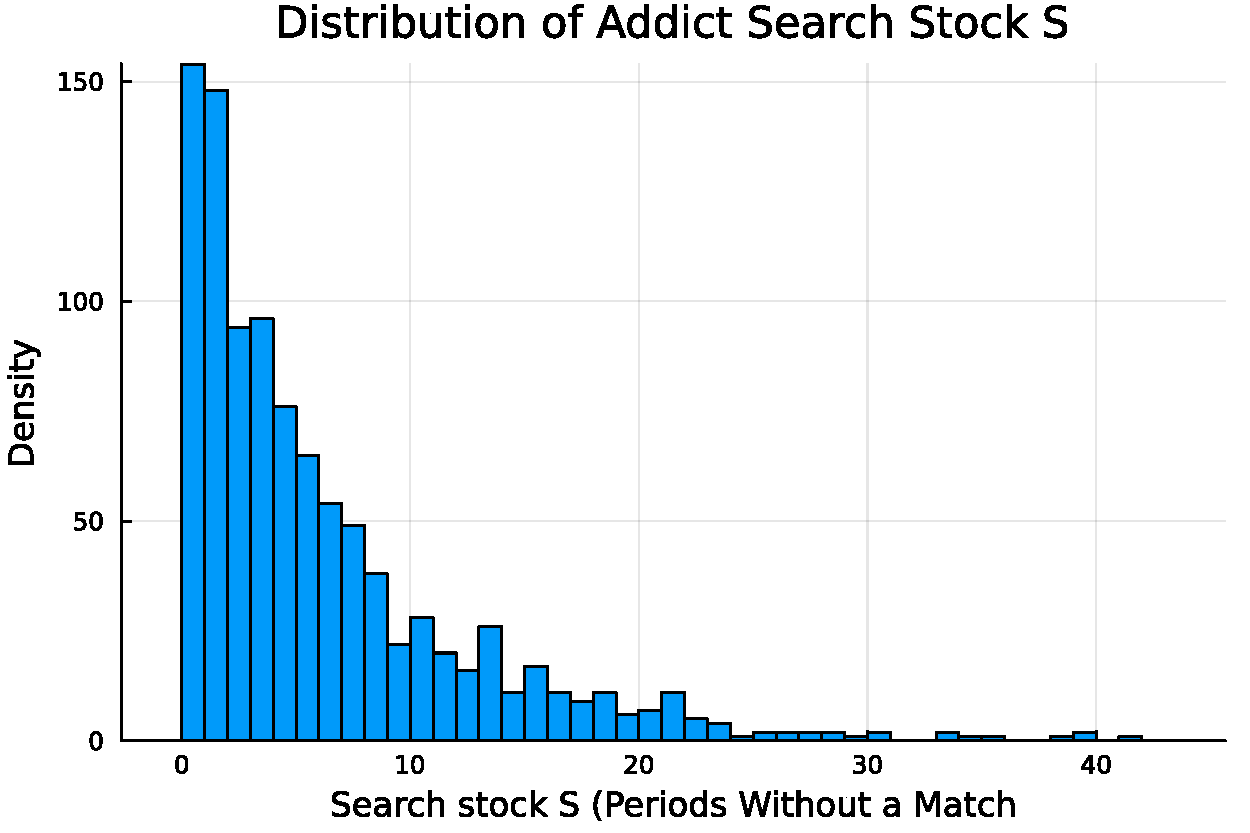
\includegraphics[width = 0.45\linewidth]{../figures/addict_search_stock_distribution.pdf}
    \hfill
    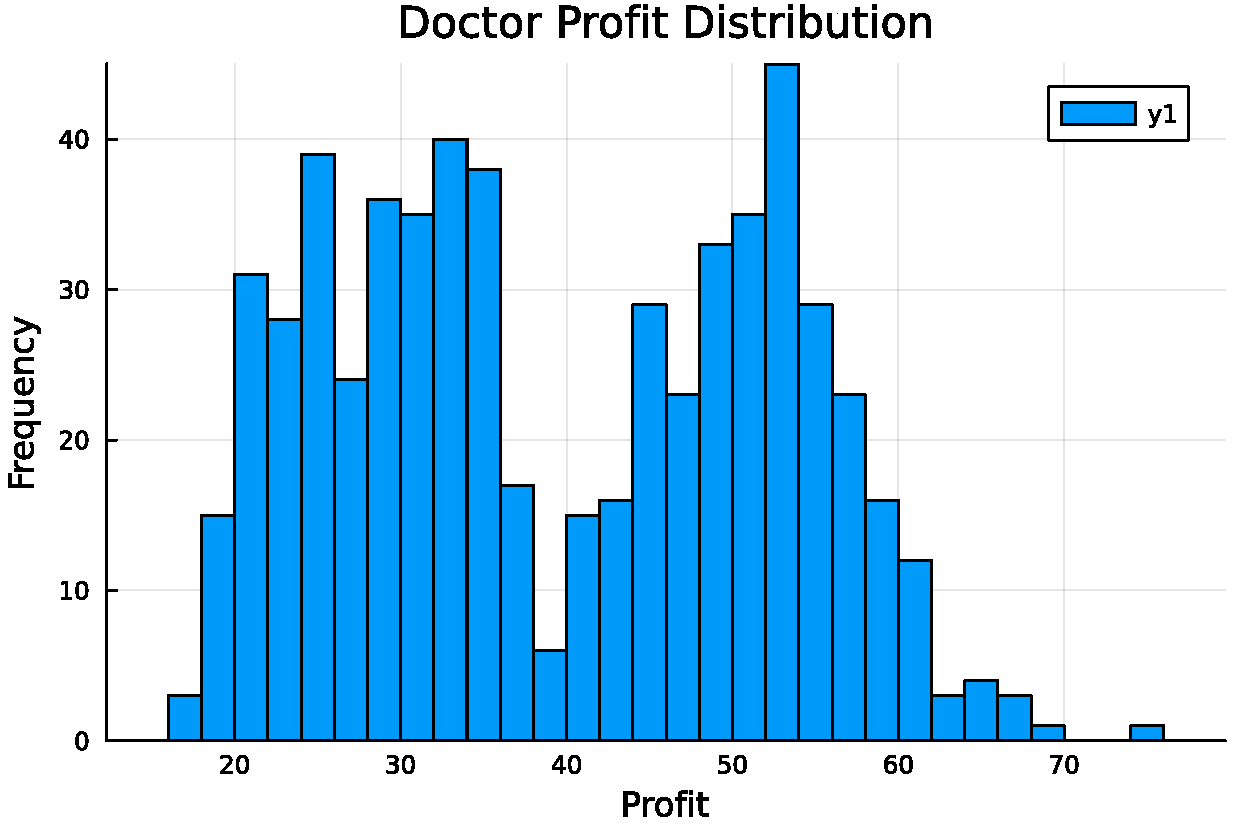
\includegraphics[width = 0.45\linewidth]{../figures/doctor_profit_distribution.pdf}
    \caption{Distributions of Addict Search Stock and Doctor Profit}
    \label{fig:distributions}
  \end{figure}
\end{frame}

\begin{frame}{Results (Cont.)}
  \centering
  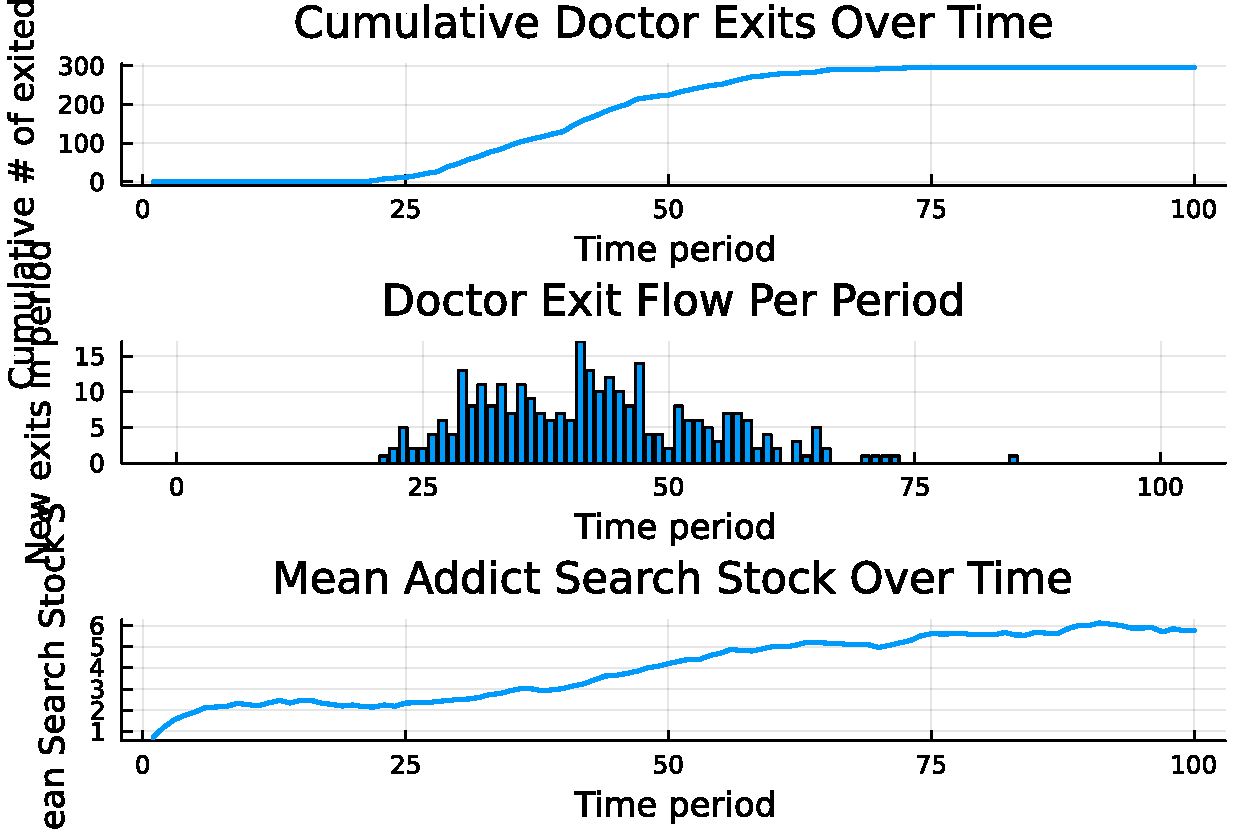
\includegraphics[width=0.7\linewidth]{../figures/doctor_exits_over_time.pdf}
\end{frame}

\begin{frame}{Counterfactual Results}
  \begin{figure}
    \centering
    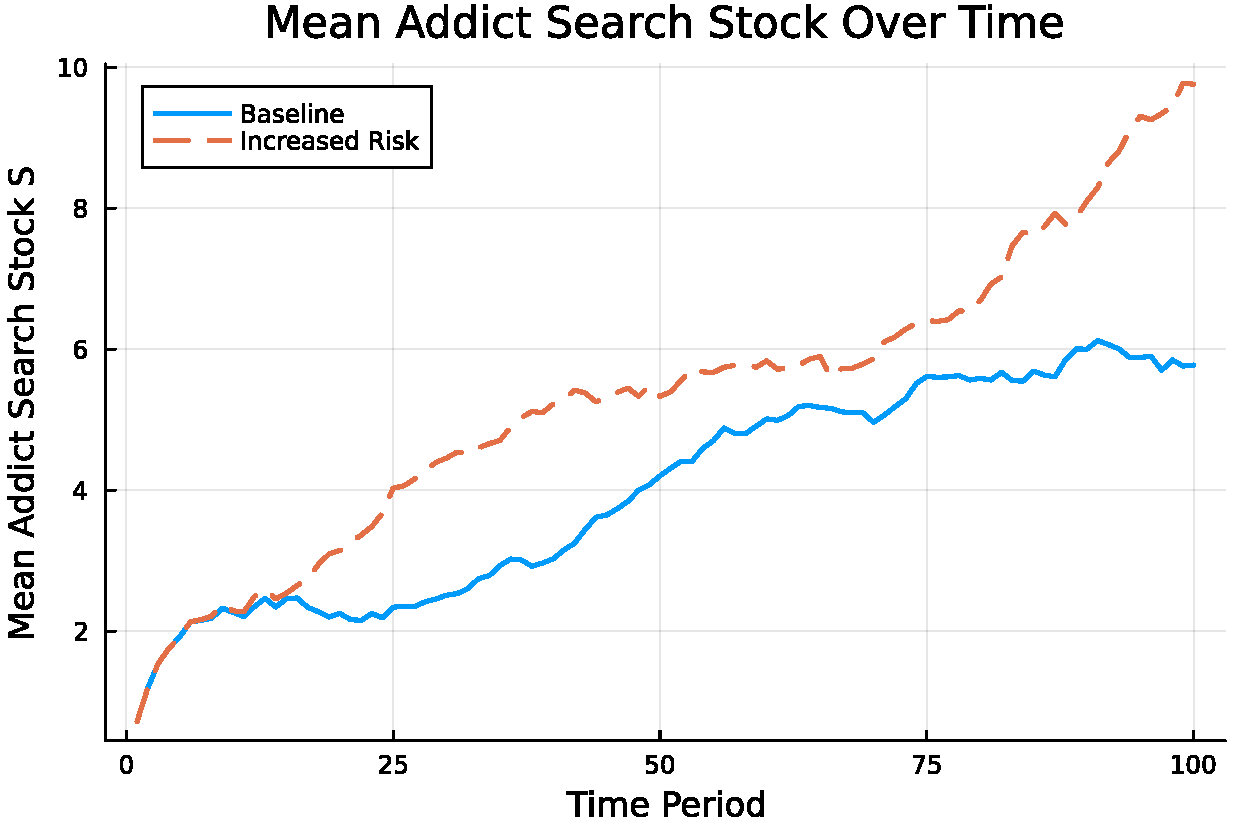
\includegraphics[width = 0.45\linewidth]{../figures/counterfactual_addict_search_stock.pdf}
    \hfill
    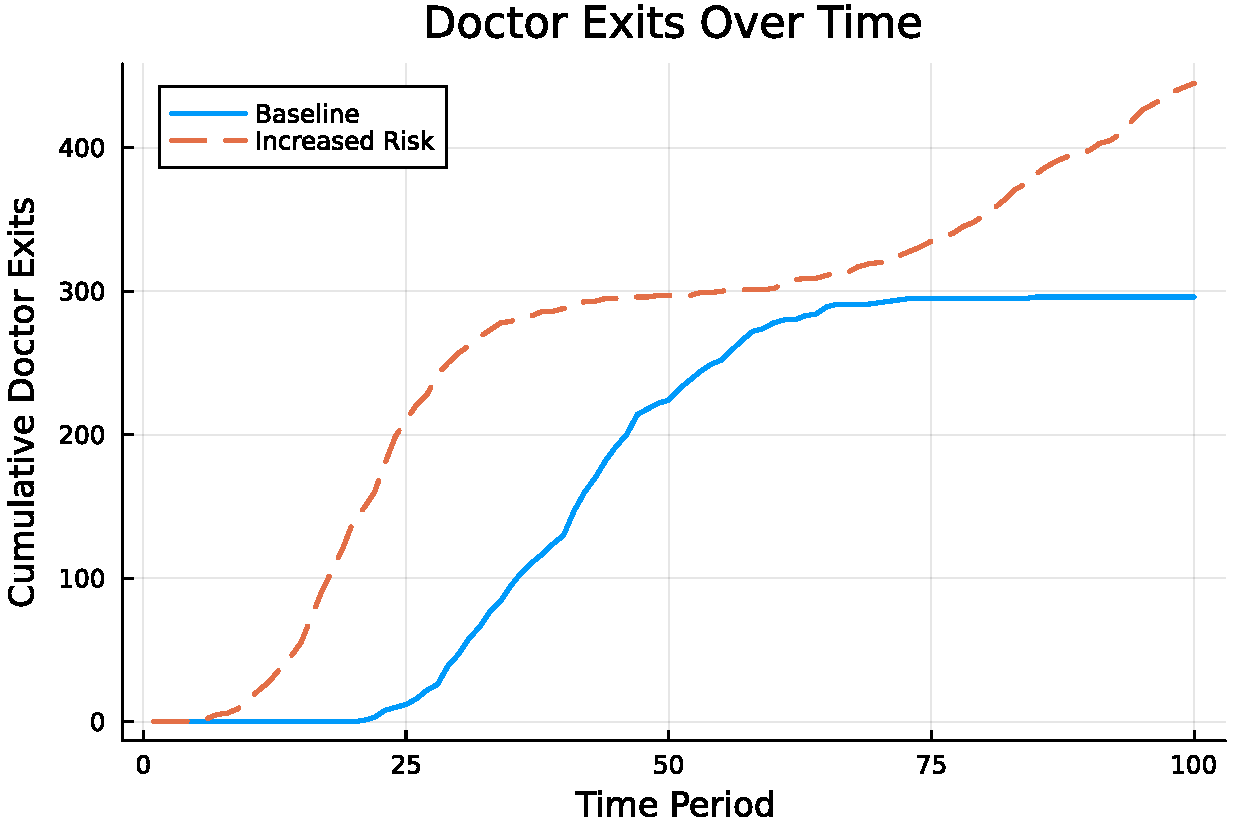
\includegraphics[width = 0.45\linewidth]{../figures/counterfactual_doctor_exits.pdf}
    \caption{Counterfactual Distributions of Addict Search Stock and Doctor Profit}
    \label{fig:counterfactual_distributions}
  \end{figure}
\end{frame}

% ============================================================
% 7) CONCLUSION
% ============================================================
\section{Conclusion and Next Steps}

\begin{frame}{Next Steps}
  \begin{itemize}
    \item Calibrate to actual data
    \item Build on basis through dynamic types and learning
    \item Explore additional policy interventions
  \end{itemize}
\end{frame}

\begin{frame}{Conclusion}
  \begin{itemize}
    \item This paper develops a dynamic programming model to analyze the interaction between addict search behavior and physician prescribing patterns.
    \item Key findings indicate that policy interventions targeting physician behavior can significantly impact addict search strategies, with important implications for public health policy.
    \item Policy makers should consider the dynamic responses of both addicts and physicians when designing interventions to address prescription drug abuse.
    \item Future work will focus on calibrating the model to real-world data and exploring additional policy scenarios to inform effective interventions.
  \end{itemize}
\end{frame}

\begin{frame}{Thank You}
  \centering
  \Large Questions?
\end{frame}

\end{document}
